% Canonical editable hybrid figure; see method_redesign_brief.md and assets/method_assets.json.
% At 5.5 in, the smallest label remains above 8 pt.
\begin{tikzpicture}[x=1cm,y=1cm,>=Latex,
  font=\sffamily\fontsize{8.6}{10.2}\selectfont,text=ink,
  tile/.style={draw=ink!30,fill=ink!2,rounded corners=2pt,line width=.55pt,
    align=center,text width=2.70cm,minimum height=1.70cm,inner sep=4pt},
  obs/.style={tile,draw=obsblue!70,fill=obsblue!5},
  dyn/.style={tile,draw=dynorange!75,fill=dynorange!6},
  flow/.style={->,line width=.75pt,draw=ink!85},
  observation/.style={flow,draw=obsblue},
  dynamics/.style={flow,draw=dynorange},
  supervision/.style={->,line width=.65pt,dashed,draw=ink!65},
  label/.style={fill=white,inner sep=1.5pt,font=\sffamily\fontsize{8.2}{9.8}\selectfont},
  stage/.style={anchor=west,font=\sffamily\bfseries\fontsize{10}{11.5}\selectfont},
  small/.style={font=\sffamily\fontsize{8.2}{9.8}\selectfont}]
\path[use as bounding box] (0,-1.40) rectangle (13.70,9.82);

% 1. Only observed images and executed actions enter context inference.
\node[stage] at (.10,9.58) {1\quad Infer two contexts from real history};
\node[tile] (support) at (1.50,7.85) {\textbf{History frames}\\[3pt]
  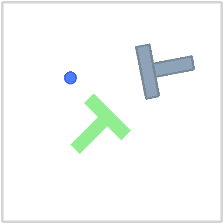
\includegraphics[width=.59cm]{figures/assets/method_pusht_frame_0.png}\hspace{2pt}%
  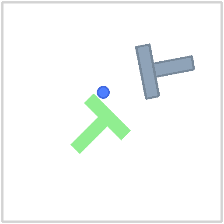
\includegraphics[width=.59cm]{figures/assets/method_pusht_frame_1.png}\hspace{2pt}%
  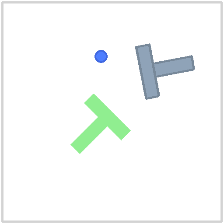
\includegraphics[width=.59cm]{figures/assets/method_pusht_frame_2.png}\\[3pt]
  $E_0$ (frozen) $\to u_S$};
\node[obs] (co) at (4.90,7.85) {\textbf{Observation $c_o$}\\[5pt]
  mean + variance\\[3pt]
  $C_o(u_S)\to c_o$};
\node[obs] (zs) at (8.30,7.85) {\textbf{Calibrate history}\\[5pt]
  $u_S\ \xrightarrow{\ A_o(\cdot,c_o)\ }\ z_S$\\[3pt]
  scale + shift};
\node[dyn] (cd) at (11.70,7.85) {\textbf{Dynamics context}\\[5pt]
  $(z_t,\Delta z_t,a_t)$\\[3pt]
  $\xrightarrow{\ \mathrm{GRU}\ }c_d$};
\draw[flow] (support) -- (co);
\draw[observation] (co) -- (zs);
\draw[flow] (zs) -- (cd);
\draw[flow] (support.north) -- ++(0,.38) -| (zs.north);
\node[label] at (4.90,9.10) {raw history features $u_S$};
\node[small,anchor=south] (past) at (11.70,9.08) {executed actions $a_S$};
\draw[dynamics] (past.south) -- (cd.north);

% 2. The same observation correction is applied to history and goal.
\node[stage] at (.10,6.45) {2\quad Imagine futures};
\node[tile] (goal) at (1.50,5.12) {\textbf{Goal image}\\[3pt]
  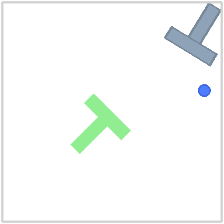
\includegraphics[width=.62cm]{figures/assets/method_pusht_frame_7.png}\\[3pt]
  $E_0$ (frozen) $\to u_g$};
\node[obs] (zg) at (4.90,5.12) {\textbf{Calibrate goal}\\[5pt]
  $u_g\ \xrightarrow{\ A_o(\cdot,c_o)\ }\ z_g$\\[3pt]
  shared $A_o$ and $c_o$};
\node[tile,minimum height=1.70cm] (rollout) at (8.30,5.12) {\textbf{LeWM predictor}\\[4pt]
  $z_t\to\hat z_{t+1}\to\cdots$\\[4pt]
  autoregressive $P$};
\node[dyn] (action) at (11.70,5.12) {\textbf{Condition actions}\\[5pt]
  $E_a(a)\xrightarrow{\ A_d\ }\tilde a$\\[3pt]
  scale + shift};
\draw[flow] (goal) -- (zg);
\draw[observation] (co.south) -- node[label,pos=.25] {$c_o$} (zg.north);
\draw[flow] (zs.south) -- node[label,pos=.56] {$z_S$} (rollout.north);
\draw[dynamics] (cd.south) -- node[label,pos=.56] {$c_d$} (action.north);
\draw[dynamics] (action) -- (rollout);
\node[small,anchor=north] (candidate) at (11.70,4.03) {candidate actions};
\draw[dynamics] (candidate.north) -- (action.south);

% 3. A real goal embedding, rather than a canonical target, drives online MPC.
\node[stage] at (.10,3.62) {3\quad Score and act};
\node[tile,text width=2.70cm,minimum height=.97cm] (score) at (8.30,2.66)
  {\textbf{Goal cost + CEM}\\[4pt]$\|\hat z_{t+K}-z_g\|_2^2/d$};
\node[tile,minimum height=.97cm] (execute) at (11.70,2.66)
  {\textbf{Execute chunk}\\[4pt]first block; then replan};
\draw[flow] (rollout.south) -- node[label,pos=.50] {$\hat z_{t+K}$} (score.north);
\draw[observation] (zg.south) |- node[label,pos=.73] {$z_g$} (score.west);
\draw[flow] (score) -- (execute);
\node[anchor=north west,align=left,text width=4.05cm,small] at (.10,3.05)
  {Real history sets the contexts.\\Weights stay fixed online.\\Latent forecasts, not video.};

% Privileged training-only targets have no path into either online context.
\draw[ink!22,line width=.55pt] (.10,1.60) -- (13.55,1.60);
\node[stage] at (.10,1.22) {Offline supervision only};
\node[anchor=west,small] at (5.15,1.22) {Canonical paired targets are unavailable during deployment.};
\node[draw=ink!35,fill=ink!3,rounded corners=2pt,align=center,text width=3.0cm,
  minimum height=.89cm,inner sep=4pt] (reference) at (1.74,.22)
  {Canonical renders\\frozen $E_0\to z^*$};
\node[align=center,text width=3.8cm,minimum height=.89cm] (alignment) at (6.30,.22)
  {\textbf{Latent alignment}\\$\operatorname{mse}(A_o(u_t,c_o),z_t^*)$};
\node[align=center,text width=3.8cm,minimum height=.89cm] (prediction) at (11.39,.22)
  {\textbf{Next-step prediction}\\$\operatorname{mse}(\hat z_{t+1},z_{t+1}^*)$};
\draw[supervision] (reference.east) -- (alignment.west);
\draw[supervision] (reference.south) -- ++(0,-.27) -| (prediction.south);
\node[small,anchor=west] at (.10,-1.00)
  {Blue: observation calibration.\quad Orange: action/dynamics conditioning.\quad Dashed: training targets.};
\end{tikzpicture}
